
\chapter{Design and Implementation}
\label{cha:implementation}

Exponential values for priorities, check http://www.yakyma.com/2012/05/why-progressive-estimation-scale-is-so.html


\section{Decomposition Algorithm}

Decomposition describes the task of grouping data fields into services. Achieving a good solution according to the defined Coupling Criteria as described in \ref{sec:decompositionRequirements} requires a non trivial algorithm. This section documents the evaluation process for such an algorithm.

\subsection{Approach \#1: Clustering of a Weighted Undirected Graph}
\label{subsec:approach1_graph}

Our first approach to solve the decomposition problem was a clustering or community algorithm applied on a weighted, undirected graph.

Every data field in the model is represented by a node. Edges define a relationship between two data fields. The weight on each edge shows how \textit{close} or \textit{cohesive} two fields are. The higher the weight, the more likely they should belong to the same service. Figure \ref{fig:weighted_graph} shows an abstract example of such a graph.

\begin{minipage}[t]{0.5\textwidth}
	Figure \ref{fig:graph_approach} outlines a solution sketch for this approach. User representations such as class diagrams or use cases are imported. The \textit{importer} component extracts the data fields and the occurences of coupling, called Coupling Criteria Instances, in this model and stores this information into the database.
	
	The \textit{Solver} then creates all vertices from the data fields and builds edges between them according to the stored Coupling Criteria instances. This task is complex for the following reasons:
	
	\begin{enumerate}
		\item Coupling Criteria are not homogeneous as described in Section \ref{subsec:couplingCriteriaTypes}. 
		%TODO: write first about types before completing this item. Mention distance, closeness and cumulative criteria
		
		\item All Coupling Criteria information is reduced to a single number with one single unit of measurement. An increase of the weight for one Criteria automatically changes the relative importance of that CC to others.
		
		\item To allow the user to define the specific requirements of his system, priorities per Coupling Criteria can optionally be defined to influence the weights of each Coupling Criteria instance.
	\end{enumerate}
	
	The \textit{Clustering Algorithm} then analyzes the graph and creates clusters of data fields so that as few edges as possible need to be cut.
	
	\begin{figure}[H]
		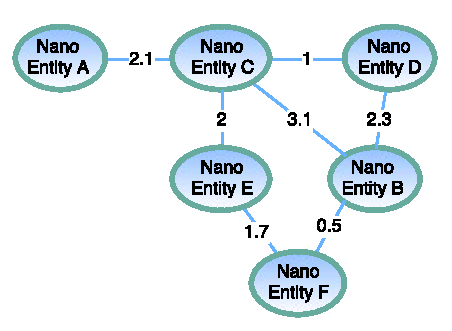
\includegraphics[scale=1.0]{diagrams/weighted_graph.pdf}
		\caption{Example of a Weighted Graph}
		\label{fig:weighted_graph}
	\end{figure}

\end{minipage}
\begin{minipage}[t]{0.5\textwidth}
	\begin{figure}[H]
		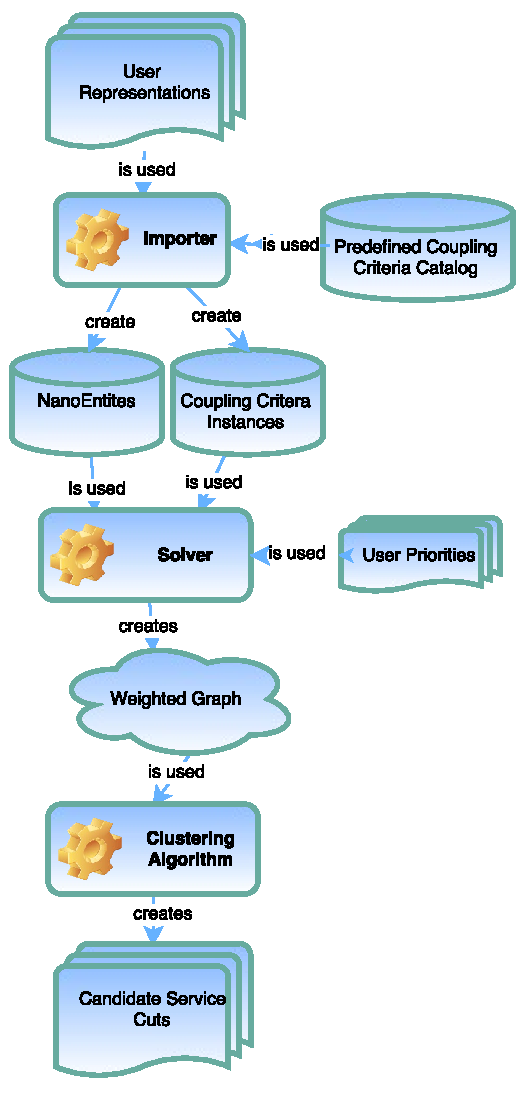
\includegraphics[scale=1.0]{diagrams/graph_approach.pdf}
		\caption{Solution Sketch for a Weighted Graph with a Clustering Algorithm}
		\label{fig:graph_approach}
	\end{figure}
\end{minipage}

A detailed evaluation of clustering algorithms is document in Appendix \ref{appendix:graphClustering}. We decided to do a first assessment of this approach using the MCL\cite{mcl} and Girvan-Newman\cite{girvanNewman} algorithms. Both algorithms are implemented as plugins of the Gephi\cite{gephi} platform and can be extracted as \gls{JAR} files.

\subsubsection{Practical Assessment of the Graph Clustering Approach}

To assess the graph approach we use a simple booking domain model. In Figure \ref{fig:clusteringBookingSimple} the MCL algorithm was tested using the booking model with all Coupling Criteria priorities set to zero except the \textit{Identity \& Lifecycle Commonality} Criteria. Consequently the visualized services contain one entity each. The entities can be identified as \textit{Customer}, \textit{Article} and \textit{Booking}.

\begin{figure}[H]
	\begin{center}
		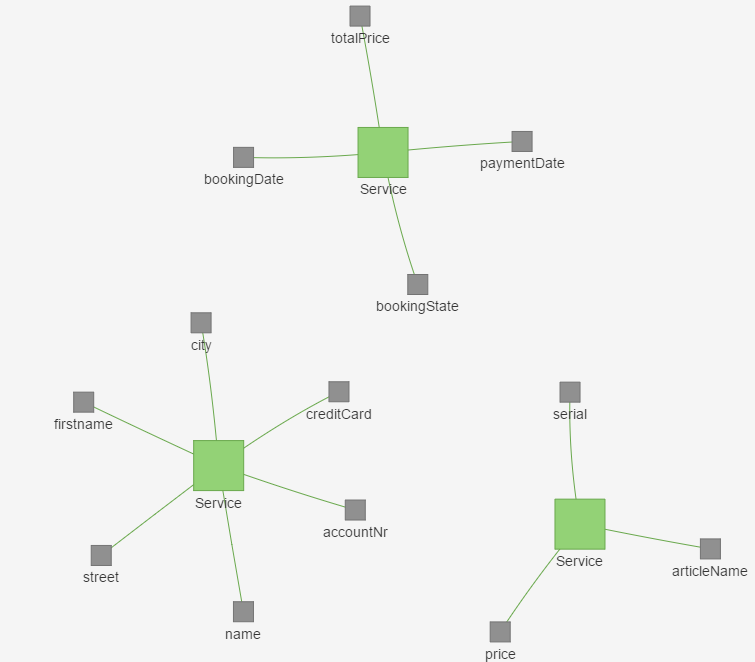
\includegraphics[scale=0.8]{images/booking_entities.png}
	\end{center}
	\caption{Clustering of a simple Booking example.}
	\label{fig:clusteringBookingSimple}
\end{figure}


Figure \ref{fig:clusteringBooking} demonstrates the result of the MCL algorithm with user stories of the Booking domain added. 

\begin{figure}[H]
	\begin{center}
		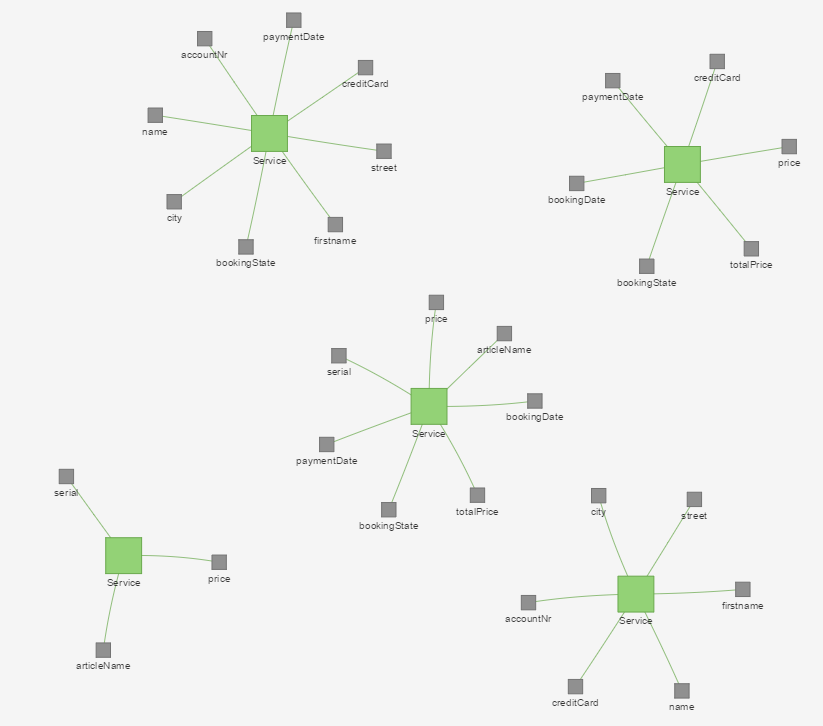
\includegraphics[scale=0.7]{images/booking_entities_mcl.png}
	\end{center}
	\caption{Booking Example enhanced with User Stories.}
	\label{fig:clusteringBooking}
\end{figure}

Obviously this is not the expected result. The requirement that a data field should be once and only once grouped to a Service is not met and the meaning of each Service can't be interpreted. %TODO noch etwas holprig...


\subsubsection{Discussion}
Theoretical assessment %TODO


\subsection{Approach \#2: Rating of possible Service Cuts}

During sprint 2 we conducted a feasibility assessment with a professor of mathematics of the graph based approach as documented in Appendix \ref{sec:feasibilityAssessment}. The result of the assessment is the idea to create a set of all possible service cuts and rate the cuts isolated per Coupling Criteria. The approach is illustrated in Figure \ref{fig:setProcess}.

\begin{figure}[H]
	\begin{center}
		\includegraphics[scale=0.45]{diagrams/scoring_process.png}
	\end{center}
	\caption{Approach \#2: Set Rating}
	\label{fig:setProcess}
\end{figure}

This approach is processed in three steps:

\begin{description}
	\item[Partitioning] Based on the data fields, a set of all possible candidate service cuts is calculated. This includes every theoretically possible service cut for every number of services. For practical usage, this step needs to be optimized. 
	\item[Assessment] For all Coupling Criteria a processor assesses all service cuts with a score describing how well the criteria's requirements are met. The score is a number between 0 and 10, while 10 means that all requirements are perfectly satisfied. 
	\item[Evaluation] The user optionally defines priorities how important each Criteria is for his system. The priorities are defined with approximately exponential numbers like the Fibonacci sequence. These priorities are applied on the service cut scores. The resulting best candidate cut is then presented to the user.
\end{description}

\subsubsection{Discussion}

An advantage of this approach is that each relevant step is clearly separated and can thus be analyzed, debugged and visualized better than in the graph based approach. The assessment and score calculation is done separately for every cut and for every Coupling Criteria. Each Criteria processor needs to score candidate cuts with a uniform scoring range. 

The weak point is the partitioning process. Theoretically every possible set of services where each data field is contained in one and only one Service is a candidate cut. In mathematics this is described as the \textit{partition of a set}\cite{partitionOfASet} problem. The Bell number $B_n$ defines the amount of possible partitions: 


\begin{displaymath}
B_{n+1}=\sum_{j=0}^n {n\choose j} B_j
\end{displaymath}

For the Service Cutter $n$ is the number of data fields, so the number of possible service cuts for $n=20$ data fields is $51'724'158'235'372$\footnote{We don't show the number for the required $2000$ data fields for lack of space in the document.}.

The Bell number includes cuts for $1 - n$ number of Services. In the context of a software system only certain numbers of Services are realistic. The \textit{Stirling numbers of the second kind} calculate the Bell number for a given number of sets $k$:

\begin{displaymath}
\left\{ {n \atop k}\right\} = \frac{1}{k!}\sum_{j=0}^{k} (-1)^{k-j} \binom{k}{j} j^n
\end{displaymath}

For $n=20$ data fields and $k=4$ Services the equation results in $45'232'115'901$ possible cuts. For $k=6$ its already $4'306'078'895'384$.

During a discussion with our industry partner and supervisor documented in Appendix \ref{sec:status22102015}, we decided that the Service Cutter should be able to process system models with up to 2000 data fields. We therefore concluded in the same meeting that this approach is not practicable without a heuristic approach of finding a small set of relevant candidate cuts. 

A possible heuristic approach is to take one or a few Coupling Criteria information about the system into account for finding Service Candidates. A simple example would be to only analyze cuts where data fields of the same entity are not split across services so that only entities and not it's data fields need to be considered.

As we tried to find a heuristic approach to calculate candidate cuts, we discovered a new idea for the composition algorithm described in the next approach. 

\subsection{Approach \#3: Constructing Services - a Heuristic Approach}

(Notes only)
Idee:

Distanzkriterien: Umso mehr Services umso besser die Lösung (Nanoservices)
Nähekriterien: Umso weniger Services umso besser die Lösung (Monolith)

Die richtige Anzahl Services ist eine kritische Dimension der Lösung, welche unter anderem aber von vielen externen (z.B Infrastruktur) Faktoren abhängt. Entscheidung: Die Verantwortung für das bestimmen der Anzahl Services an den User auslagern.

Nun ist es möglich eine bestimmte Anzahl Services zu füllen. Dazu kann ein heuristischer, empirischer Algorithmus mit intelligentem Rütteln genommen werden. 
Jede Verbindung von zwei Feldern wird von jedem CC mit einer einheitlichen Einheit bewertet. Dadurch kann einfach bestummen werden, wie gut ein Feld in ein Topf passt. Alle Töpfe werden gefüllt (wenn es nirgends passt in den kleinsten Topf). Danach wird angefangen Feldern die am wenigsten passen in einen anderen Topf zu werfen.
Der Algorithmus kann beliebig(?) weiterlaufen und optimieren. Wenn der Algorithmus gut funktioniert, kann man während der Optimierung auch die Gewichtung anpassen und schauen was damit passiert.
Idee: Snapshots machen von Status bevor eine Gewichtung angepasst wird.
Idee: Am Anfang 5 Minuten durchlaufen, 10 Vorschläge ausarbeiten und dann den user entscheiden lassen auf welchen er weiter optimieren will (?) Evtl. kann auch der Algorithmus entscheiden indem er die lösungen vergleicht? 

Weitere Idee: Aufsplitten auf logische (A) und physische (B) Kriterien und Decomposition mode? Kann der Algorithmus in zwei Schritten geschehen? Bzw. lösen wir eigentlich 2 Probleme (Logisch \& Physisch) auf einmal?

\section{Prototype} 

\subsection{Design}

\subsection{Technology}


\begin{minipage}[t]{0.5\textwidth}
	The Service Cutter is implemented as a three tier application.
	
	The first tier is the web \textit{browser} of the user. The single-page application is based on AngularJS\cite{angularjs} and uses a template based on Bootstrap\cite{bootstrap}. A REST API provides access to the Editor tier.
	
	The \textit{Editor} component is a web application based on the JHipster\cite{jhipster} framework. It provides the use the possibility to import this domain information using a JSON upload and feeds this information into the Engine. All security and user interface aspects are handled in this layer.
	
	The Engine is the isolated component that holds all the code to calculate service decomposition suggestions. It is also based on Spring technologies and provides a REST web service. The Engine does not provide any security measures and it is therefore necessary to restrict access to the Engine. We recommend to achieve this using a Docker\cite{docker} internal network as described in Section \ref{subsec:infrastructure}.
	
\end{minipage}
\begin{minipage}[t]{0.5\textwidth}
	\begin{figure}[H]
		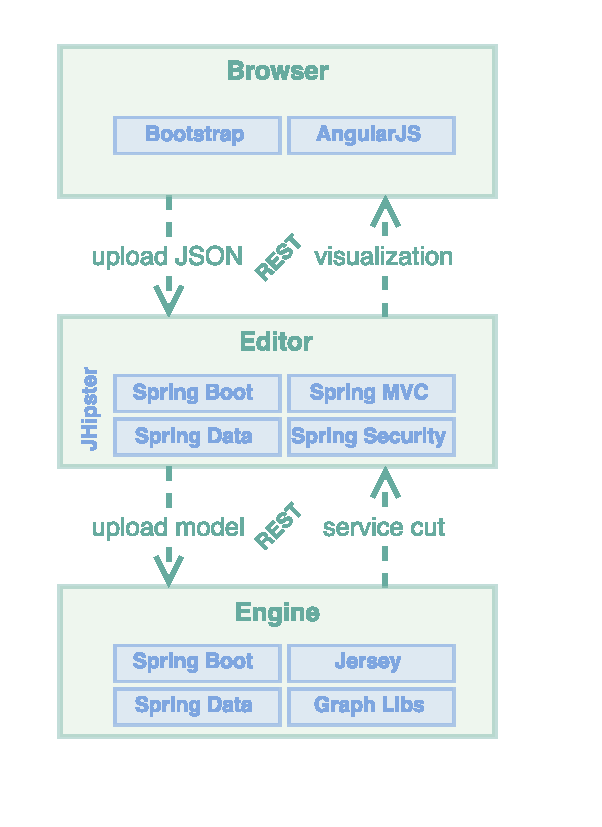
\includegraphics[scale=1]{diagrams/Technologies.pdf}
		\caption{Technology overview}
		\label{fig:technologies}
	\end{figure}
\end{minipage}


\subsection{Infrastructure}
\label{subsec:infrastructure}

\subsection{Information Security}

The web application is secured using an authentication and authorization implementation. Any other internal components such as the database or web services are hidden behind the servers firewall and therefore do not need any special security measures.

The uploaded data models are initially shared amongst all registered users.

\subsection{User Interface}

The base layout is responsive and adapts to smaller screens such as smartphones. However the tool is mostly used on devices such as laptops and the controls are therefore optimized for use on screens that are at least 15 inches wide and used with a mouse and a keyboard.


\bigskip
After covering the important design and implementation aspects, the next chapter assesses the built solution described in this chapter against the defined requirements.
